\documentclass[]{article}
\usepackage{lmodern}
\usepackage{amssymb,amsmath}
\usepackage{ifxetex,ifluatex}
\usepackage{fixltx2e} % provides \textsubscript
\ifnum 0\ifxetex 1\fi\ifluatex 1\fi=0 % if pdftex
  \usepackage[T1]{fontenc}
  \usepackage[utf8]{inputenc}
\else % if luatex or xelatex
  \ifxetex
    \usepackage{mathspec}
    \usepackage{xltxtra,xunicode}
  \else
    \usepackage{fontspec}
  \fi
  \defaultfontfeatures{Mapping=tex-text,Scale=MatchLowercase}
  \newcommand{\euro}{€}
\fi
% use upquote if available, for straight quotes in verbatim environments
\IfFileExists{upquote.sty}{\usepackage{upquote}}{}
% use microtype if available
\IfFileExists{microtype.sty}{%
\usepackage{microtype}
\UseMicrotypeSet[protrusion]{basicmath} % disable protrusion for tt fonts
}{}
\usepackage[margin=1in]{geometry}
\usepackage{color}
\usepackage{fancyvrb}
\newcommand{\VerbBar}{|}
\newcommand{\VERB}{\Verb[commandchars=\\\{\}]}
\DefineVerbatimEnvironment{Highlighting}{Verbatim}{commandchars=\\\{\}}
% Add ',fontsize=\small' for more characters per line
\usepackage{framed}
\definecolor{shadecolor}{RGB}{248,248,248}
\newenvironment{Shaded}{\begin{snugshade}}{\end{snugshade}}
\newcommand{\KeywordTok}[1]{\textcolor[rgb]{0.13,0.29,0.53}{\textbf{{#1}}}}
\newcommand{\DataTypeTok}[1]{\textcolor[rgb]{0.13,0.29,0.53}{{#1}}}
\newcommand{\DecValTok}[1]{\textcolor[rgb]{0.00,0.00,0.81}{{#1}}}
\newcommand{\BaseNTok}[1]{\textcolor[rgb]{0.00,0.00,0.81}{{#1}}}
\newcommand{\FloatTok}[1]{\textcolor[rgb]{0.00,0.00,0.81}{{#1}}}
\newcommand{\CharTok}[1]{\textcolor[rgb]{0.31,0.60,0.02}{{#1}}}
\newcommand{\StringTok}[1]{\textcolor[rgb]{0.31,0.60,0.02}{{#1}}}
\newcommand{\CommentTok}[1]{\textcolor[rgb]{0.56,0.35,0.01}{\textit{{#1}}}}
\newcommand{\OtherTok}[1]{\textcolor[rgb]{0.56,0.35,0.01}{{#1}}}
\newcommand{\AlertTok}[1]{\textcolor[rgb]{0.94,0.16,0.16}{{#1}}}
\newcommand{\FunctionTok}[1]{\textcolor[rgb]{0.00,0.00,0.00}{{#1}}}
\newcommand{\RegionMarkerTok}[1]{{#1}}
\newcommand{\ErrorTok}[1]{\textbf{{#1}}}
\newcommand{\NormalTok}[1]{{#1}}
\usepackage{graphicx}
\makeatletter
\def\maxwidth{\ifdim\Gin@nat@width>\linewidth\linewidth\else\Gin@nat@width\fi}
\def\maxheight{\ifdim\Gin@nat@height>\textheight\textheight\else\Gin@nat@height\fi}
\makeatother
% Scale images if necessary, so that they will not overflow the page
% margins by default, and it is still possible to overwrite the defaults
% using explicit options in \includegraphics[width, height, ...]{}
\setkeys{Gin}{width=\maxwidth,height=\maxheight,keepaspectratio}
\ifxetex
  \usepackage[setpagesize=false, % page size defined by xetex
              unicode=false, % unicode breaks when used with xetex
              xetex]{hyperref}
\else
  \usepackage[unicode=true]{hyperref}
\fi
\hypersetup{breaklinks=true,
            bookmarks=true,
            pdfauthor={@tribetect},
            pdftitle={Investigating the exponential distribution and comparing it with the Central Limit Theorem},
            colorlinks=true,
            citecolor=blue,
            urlcolor=blue,
            linkcolor=magenta,
            pdfborder={0 0 0}}
\urlstyle{same}  % don't use monospace font for urls
\setlength{\parindent}{0pt}
\setlength{\parskip}{6pt plus 2pt minus 1pt}
\setlength{\emergencystretch}{3em}  % prevent overfull lines
\setcounter{secnumdepth}{0}

%%% Use protect on footnotes to avoid problems with footnotes in titles
\let\rmarkdownfootnote\footnote%
\def\footnote{\protect\rmarkdownfootnote}

%%% Change title format to be more compact
\usepackage{titling}

% Create subtitle command for use in maketitle
\newcommand{\subtitle}[1]{
  \posttitle{
    \begin{center}\large#1\end{center}
    }
}

\setlength{\droptitle}{-2em}
  \title{Investigating the exponential distribution and comparing it with the
Central Limit Theorem}
  \pretitle{\vspace{\droptitle}\centering\huge}
  \posttitle{\par}
  \author{@tribetect}
  \preauthor{\centering\large\emph}
  \postauthor{\par}
  \predate{\centering\large\emph}
  \postdate{\par}
  \date{August 18, 2015}



\begin{document}

\maketitle


\section{Overview}\label{overview}

In a few (2-3) sentences explain what is going to be reported on

We investigated the distribution of averages of 40 exponentials doing
1000 simulations.

\section{Simulations}\label{simulations}

Include English explanations of the simulations you ran, with the
accompanying R code. Your explanations should make clear what the R code
accomplishes.

\begin{enumerate}
\def\labelenumi{\arabic{enumi}.}
\itemsep1pt\parskip0pt\parsep0pt
\item
  The exponential distribution was simulated in R with rexp(n, lambda)
  where lambda is the rate parameter. The mean of exponential
  distribution is 1/lambda and the standard deviation is also 1/lambda.
\item
  Lambda was set = 0.2 for all of the simulations.
\item
  Set number of simulations to 1000: variable, `nosim'.
\end{enumerate}

\begin{Shaded}
\begin{Highlighting}[]
\NormalTok{my_seed =}\StringTok{ }\DecValTok{512} \CommentTok{#for random number generators based simulations}
\KeywordTok{set.seed}\NormalTok{(my_seed) }

\CommentTok{# Setup the supplied quantities as variables}
\NormalTok{lambda <-}\StringTok{ }\FloatTok{0.2}
\NormalTok{samplesize <-}\StringTok{ }\DecValTok{40} \CommentTok{#size of random exponential samples }
\NormalTok{nosim =}\StringTok{ }\DecValTok{1000} \CommentTok{#number of simulations}
\NormalTok{mns =}\StringTok{ }\OtherTok{NULL} \CommentTok{#variable to store means of samples}
\end{Highlighting}
\end{Shaded}

\section{Comparing Sample Mean and Theoretical
Mean}\label{comparing-sample-mean-and-theoretical-mean}

We plot the distribution of a 1000 simulated means of sampletaken from
an exponential distribution. Size of each sample was 40.

The theoratical mean of the distribution, shown using a vertical red
line, is close to the center of the distribution of means of the
samples.

\begin{Shaded}
\begin{Highlighting}[]
\NormalTok{for (i in }\DecValTok{1} \NormalTok{:}\StringTok{ }\NormalTok{nosim) mns =}\StringTok{ }\KeywordTok{c}\NormalTok{(mns, }\KeywordTok{mean}\NormalTok{(}\KeywordTok{rexp}\NormalTok{(samplesize, lambda)))}
\KeywordTok{hist}\NormalTok{(mns, }\DataTypeTok{main =} \StringTok{"Distribution of sample means"}\NormalTok{)}
\NormalTok{theo_mean <-}\StringTok{ }\KeywordTok{mean}\NormalTok{(mns)}
\KeywordTok{abline}\NormalTok{(}\DataTypeTok{v =} \NormalTok{theo_mean, }\DataTypeTok{col =} \StringTok{"red"}\NormalTok{, }\DataTypeTok{lty =} \DecValTok{2}\NormalTok{)}
\KeywordTok{text}\NormalTok{(theo_mean -}\StringTok{ }\NormalTok{.}\DecValTok{5}\NormalTok{, }\DataTypeTok{y =} \DecValTok{230}\NormalTok{, }\DataTypeTok{labels =} \KeywordTok{paste}\NormalTok{(}\StringTok{"Theoretical Mean:"}\NormalTok{, }\KeywordTok{round}\NormalTok{(theo_mean,}\DecValTok{2}\NormalTok{)))}
\end{Highlighting}
\end{Shaded}

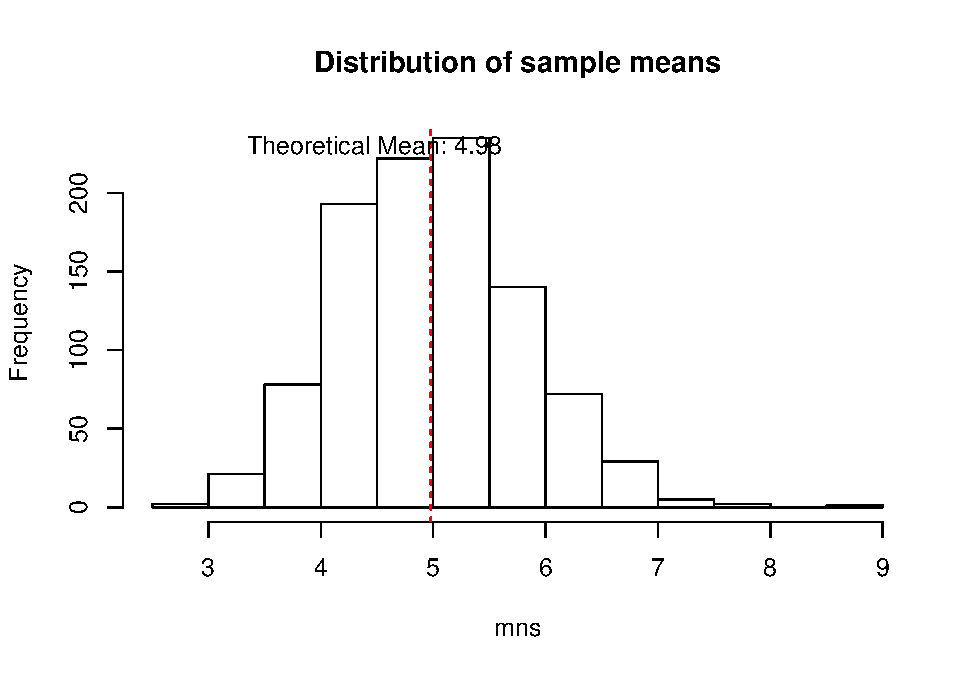
\includegraphics{Part_1_files/figure-latex/unnamed-chunk-2-1.pdf}

\section{Sample Variance versus Theoretical
Variance}\label{sample-variance-versus-theoretical-variance}

Include figures (output from R) with titles. Highlight the variances you
are comparing. Include text that explains your understanding of the
differences of the variances.

\section{Distribution}\label{distribution}

Via figures and text, explain how one can tell the distribution is
approximately normal.

\end{document}
